\documentclass[11pt]{article}
\usepackage{textcomp,geometry,graphicx,verbatim}
\usepackage{fancyhdr}
\usepackage{amsmath,amssymb,enumerate,cancel}
\usepackage{titling}
\setlength{\droptitle}{-10em}   % This is your set screw
\pagestyle{fancy}
\def\Name{Manohar Jois}
\def\Homework{4} % Homework number - make sure to change for every homework!
\def\Session{Spring 2015}

% Extra commands
\let\origleft\left
\let\origright\right
\renewcommand{\left}{\mathopen{}\mathclose\bgroup\origleft}
\renewcommand{\right}{\aftergroup\egroup\origright}
\newcommand{\N}{\mathbb{N}}
\newcommand{\Z}{\mathbb{Z}}
\newcommand{\R}{\mathbb{R}}
\newcommand{\Q}{\mathbb{Q}}
\newcommand{\C}{\mathbb{C}}
\newcommand{\p}[1]{\left(#1\right)}
\newcommand{\E}{\mathbb{E}}
\newcommand{\cov}{\text{Cov}}
\newcommand{\lhood}{\mathscr{L}}
\renewcommand{\gcd}[1]{\text{gcd}\p{#1}}
\renewcommand{\deg}[1]{\text{deg}\p{#1}}
\renewcommand{\log}[1]{\text{log}\p{#1}}
\renewcommand{\ln}[1]{\text{ln}\p{#1}}
\newcommand{\logb}[2]{\text{log}_{#1}\p{#2}}
\newcommand{\BigOh}[1]{O\p{#1}}
\newcommand{\BigOmega}[1]{\Omega\p{#1}}
\newcommand{\BigTheta}[1]{\Theta\p{#1}}
\newcommand{\asdf}{\newline\newline}

\title{CS189\ \Session\  --- Homework \Homework}
\author{\Name}
\lhead{CS189\ \Session\  Homework \Homework\ Problem \theproblemnumber,\ \Name}

\begin{document}
\maketitle
\newcounter{problemnumber}
\setcounter{problemnumber}{0}

\section*{Problem 1}
\stepcounter{problemnumber}
\begin{enumerate}[1.]
\item First we derive the gradient of $\mu_i(\beta)$ with respect to $\beta$:
$$\nabla_{\beta}\mu_i = -\frac1{(1+\exp(-\beta^Tx_i))^2}(1+\exp(-\beta^Tx_i))(-x_i) = \mu_i(1-\mu_i)x_i$$
Now we take the gradient of the negative log likelihood:
\begin{align*}
\nabla_{\beta}\ell(\beta) &= \nabla_{\beta}(\lambda\beta^T\beta) - \sum_{i=1}^n\left(\frac{y_i}{\mu_i}\nabla_{\beta}\mu_i - \frac{1-y_i}{1-\mu_i}\nabla_{\beta}\mu_i\right)\\
&= 2\lambda I\beta - \sum_{i=1}^n \left(y_i(1-\mu_i)x_i - (1-y_i)\mu_ix_i\right)\\
&= 2\lambda I\beta - \sum_{i=1}^n (y_i-\mu_i)x_i\\
&= 2\lambda I\beta - X^T(Y-\mu(\beta))
\end{align*}
\item The Hessian is just the next gradient with respect to $\beta$:
$$\nabla_{\beta}^2\ell(\beta) = 2\lambda I + X^TD(\beta)X$$
where $D(\beta)$ is simply the $n\times n$ matrix with the $i^{\text{th}}$ diagonal entry being $\mu_i(\beta)(1-\mu_i(\beta))$.
\item Newton's method updates for this gradient descent are:
\begin{align*}
\beta^{(t+1)} &= \beta^{(t)} - [\nabla_{\beta}^2\ell(\beta^{(t)})]^{-1} \nabla_{\beta}\ell(\beta^{(t)})\\
&= \beta^{(t)} - [2\lambda I + X^TD(\beta^{(t)})X]^{-1} (2\lambda I\beta^{(t)} - X^T(Y-\mu(\beta^{(t)})))
\end{align*}
\item The results to parts (a) through (d) can be viewed by running \texttt{python p1.py}. See \texttt{README} for details.\\
\begin{tabular}{cc}
$\mu^{(0)} = \mu(\beta^{(0)}) = \begin{bmatrix}(1+e^{-3})^{-1}\\(1+e^{-1})^{-1}\\(1+e^{-1})^{-1}\\(1+e^{1})^{-1}\end{bmatrix}$ & $\beta^{(1)} \approx \begin{bmatrix}-0.387\\1.404\\-2.284\end{bmatrix}$\\
$\mu^{(1)} \approx \begin{bmatrix}0.873\\0.824\\0.293\\0.220\end{bmatrix}$ & $\beta^{(2)} \approx \begin{bmatrix}-0.512\\1.453\\-2.163\end{bmatrix}$
\end{tabular}
\end{enumerate}
%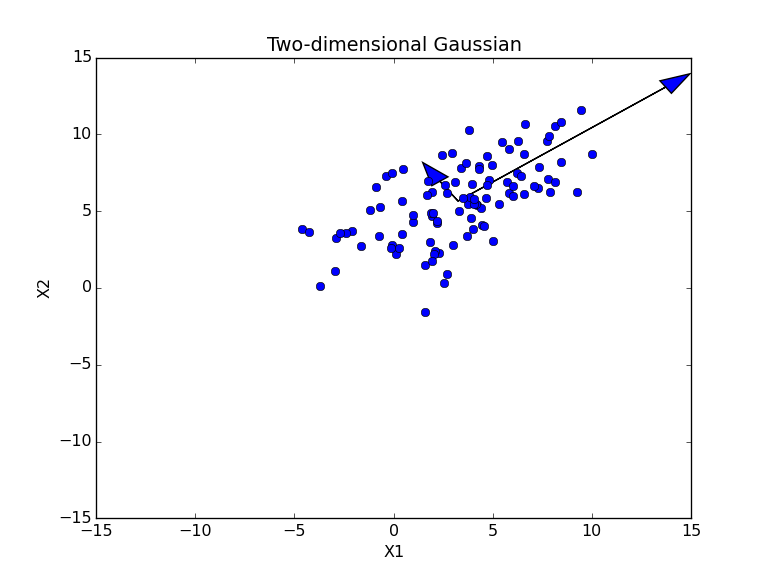
\includegraphics[scale=0.45]{images_hw3/p1d}
%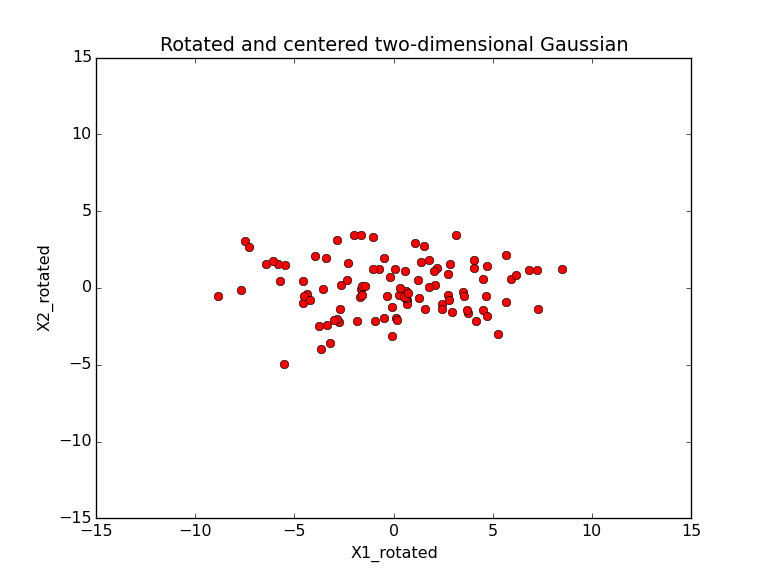
\includegraphics[scale=0.45]{images_hw3/p1e}


\newpage
\section*{Problem 2}
\stepcounter{problemnumber}
\begin{enumerate}[1.]
\item See \texttt{README} for instructions on running the code.
\item The RSS on the test set without introducing an offset term is around $4.62\cdot10^8$. When we introduce a bias so that the regression vector $\beta$ doesn't go through the origin, we get an RSS of about $2.33\cdot10^6$. The range of predicted values when not using the offset goes from around $787$ to $2995$, but when using the offset goes from about $1953$ to $2045$, which makes much more sense although about a third of this range isn't actually present in the training set (and hasn't even happened yet). This data can be viewed as output after running the code.
\item The offset coefficient $\beta_0$ was approximately $1951$.\\
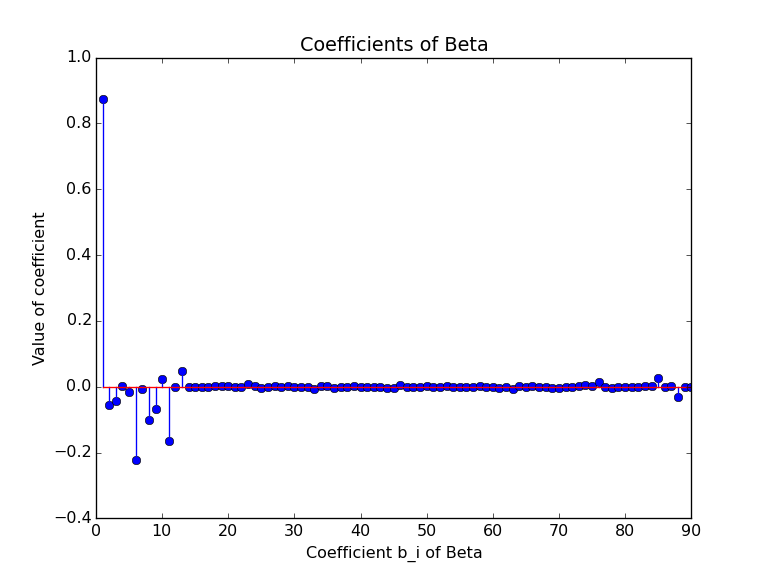
\includegraphics[scale=0.7]{images/p2}
\item The model is somewhat reasonable since the range of values produced on the test set overlaps decently with the range of the training set, and judging from the RSS our mean error on the test set is around $6$ to $7$ years. Also it makes enough sense to treat this range of years as a continuous space.
\end{enumerate}


\newpage
\section*{Problem 3}
\stepcounter{problemnumber}
\begin{enumerate}[1.]
\item Gradient descent applies to convex functions, which means we can work with the negative log-likelihood of logistic regression using $\ell_2$ regularization. We derived the gradient of this function in problem $1$.
$$\beta^{(t+1)} = \beta^{(t)}-\eta\nabla_{\beta}\ell(\beta^{(t)}) = \beta^{(t)} + \eta X^T(Y-\mu(\beta^{(t)})) - 2\eta\lambda I\beta^{(t)}$$
where $\mu(\beta)$ is again the $n\times1$ vector of all $\mu_i(\beta)=(1+\exp(-\beta^Tx_i))^{-1}$.\\
\begin{tabular}{cc}
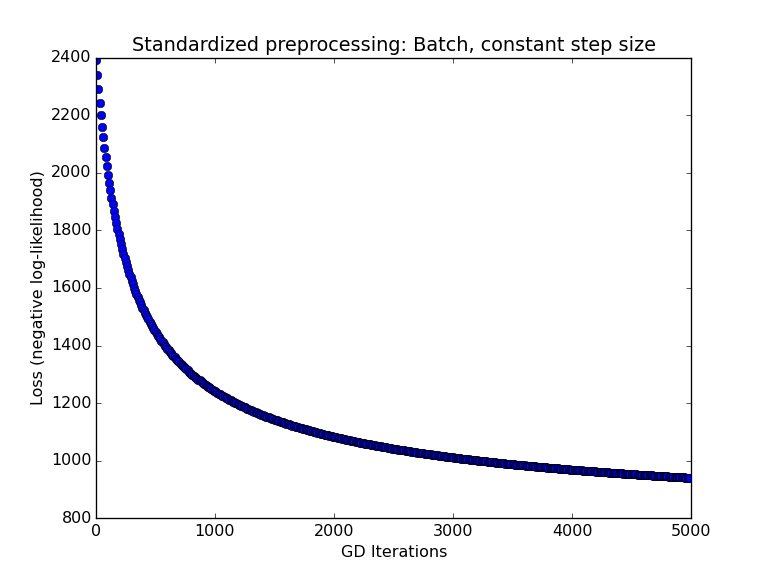
\includegraphics[scale=0.4]{images/p3_1_Standardized} & 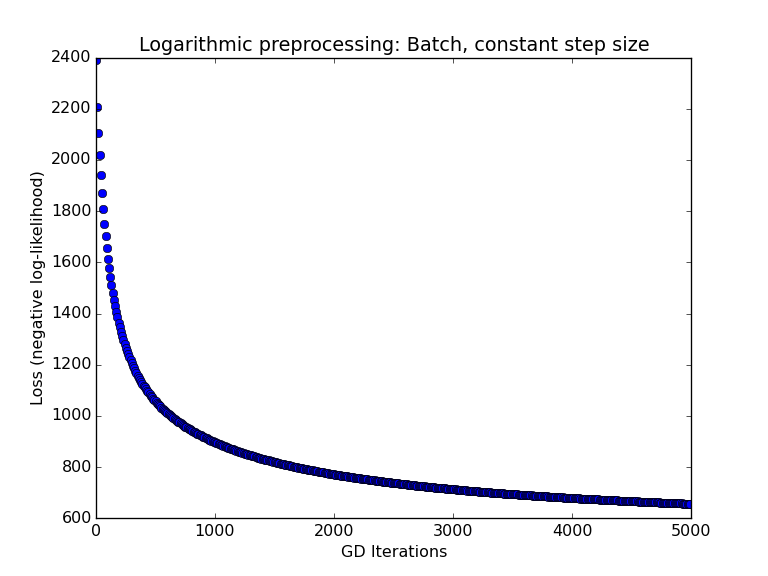
\includegraphics[scale=0.4]{images/p3_1_Logarithmic} \\
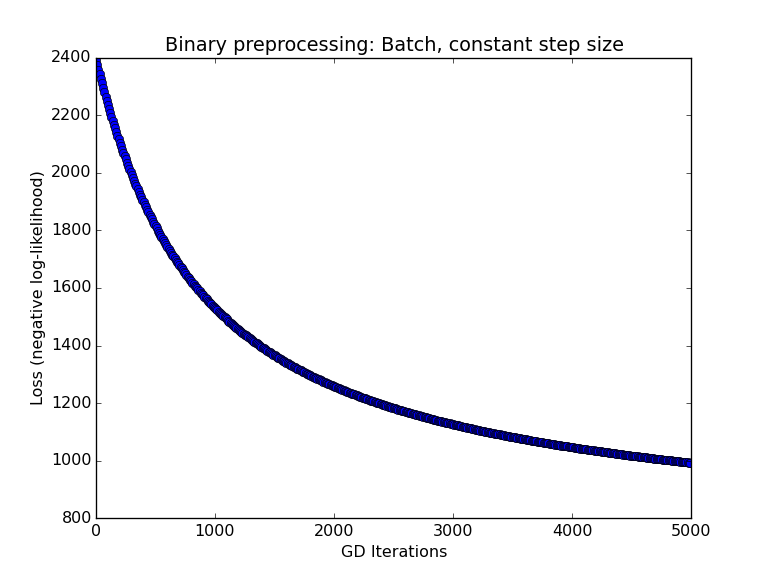
\includegraphics[scale=0.4]{images/p3_1_Binary} &
\end{tabular}
The step size was $10^{-6}$ and $\lambda=1$.
\newpage
\item The stochastic gradient descent update only chooses one data point to substitute for calculating a summation over all samples for the true gradient. Therefore the update equation uses a random $i\in[1,n]$ to calculate the next value of $\beta$:
$$\beta^{(t+1)} = \beta^{(t)}+\eta(y_i-\mu_i(\beta^{(t)}))x_i-2\eta\lambda I\beta^{(t)}$$
\begin{tabular}{cc}
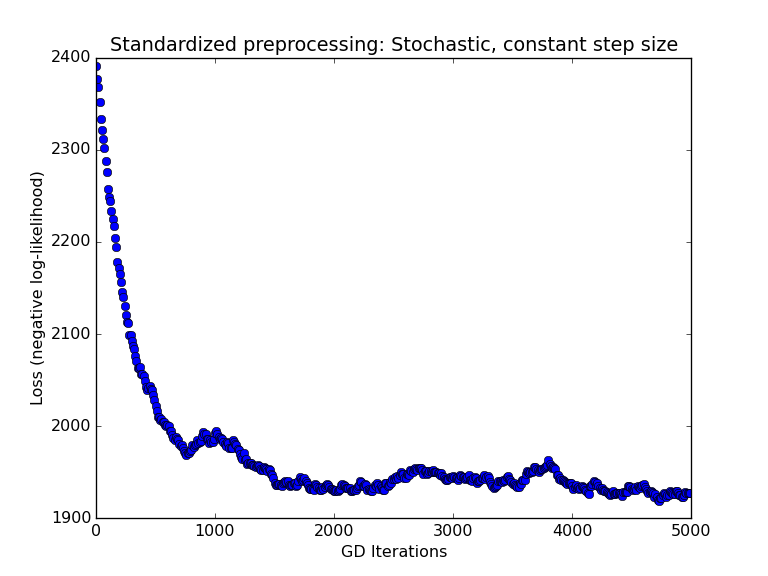
\includegraphics[scale=0.4]{images/p3_2_Standardized} & 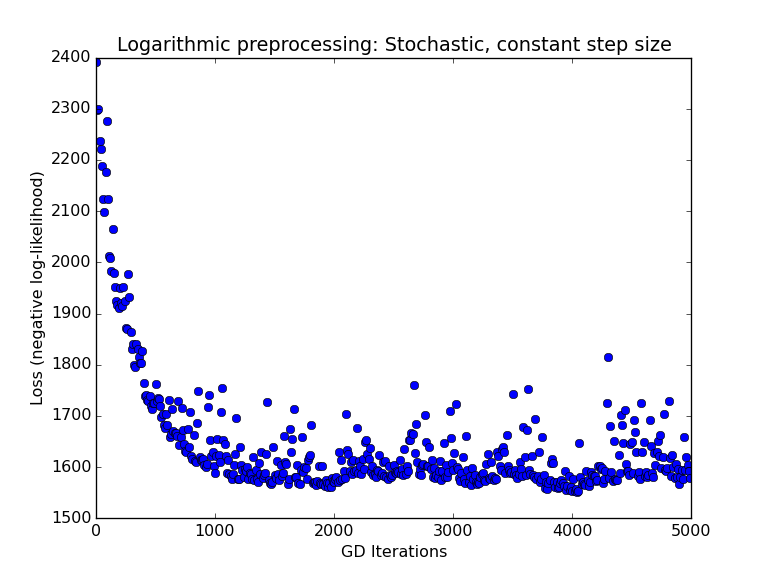
\includegraphics[scale=0.4]{images/p3_2_Logarithmic} \\
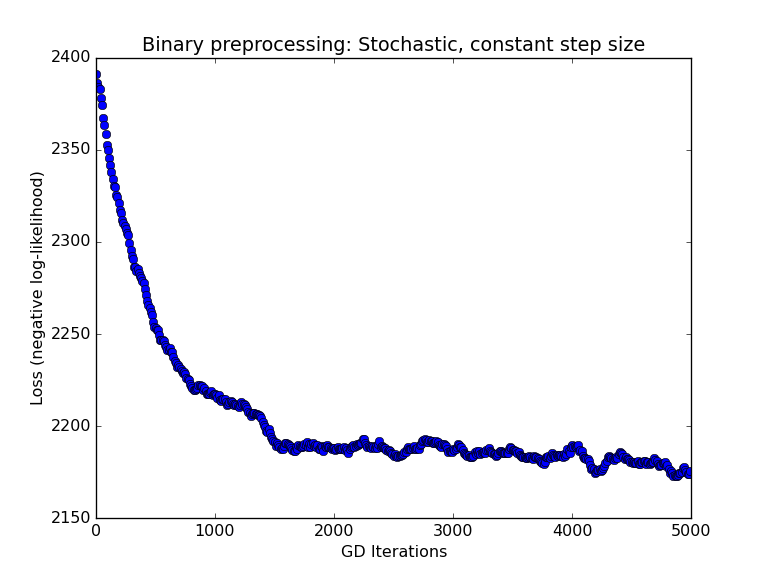
\includegraphics[scale=0.4]{images/p3_2_Binary} &
\end{tabular}
The step size was $10^{-3}$ and $\lambda=1$. In this case, we see the loss increases at times after an iteration. Even though updating based on the average of the data leads to beta values that continuously decrease loss, updating using a sample that's not very likely given your current beta vector may increase the loss. While this isn't ideal, we do it to save time on computation of the gradient and because the loss is still expected to decrease over many iterations, albeit more slowly as evidenced here.
\newpage
\item The step size was $\frac{0.2}t$ and $\lambda=1$. There seems to be a slight tradeoff between this strategy and that where $\eta$ is constant. Here we see that the iterations allow $\beta$ to converge much more quickly, but it converges to a value that produces a very slightly higher loss than before. Clearly it converges quickly because we start to value the gradient update to $\beta$ much less as the number of iterations increases. \\
\begin{tabular}{cc}
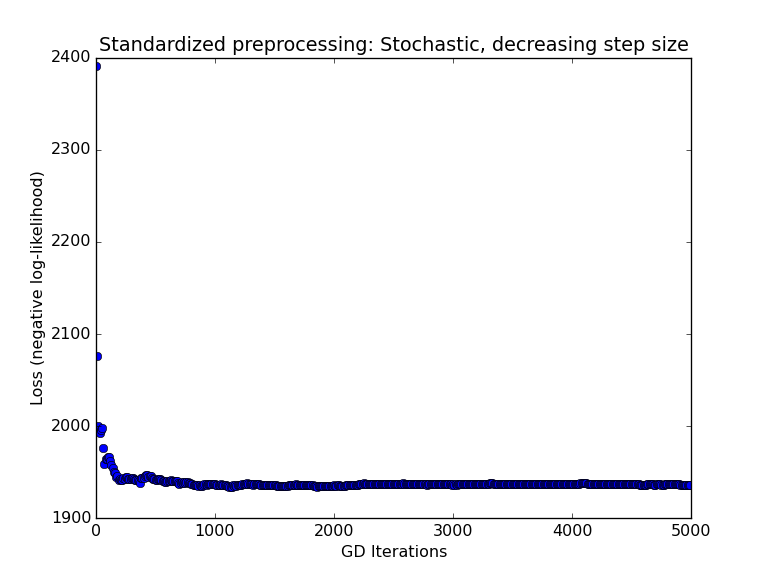
\includegraphics[scale=0.4]{images/p3_3_Standardized} & 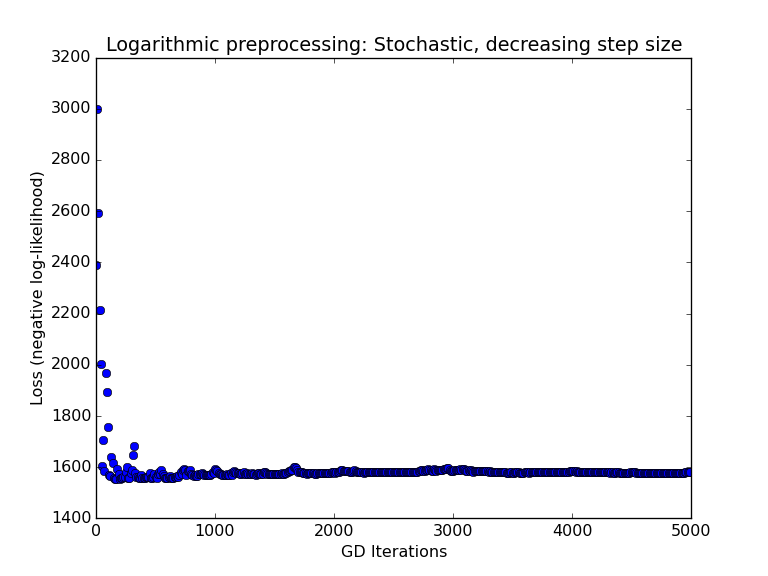
\includegraphics[scale=0.4]{images/p3_3_Logarithmic} \\
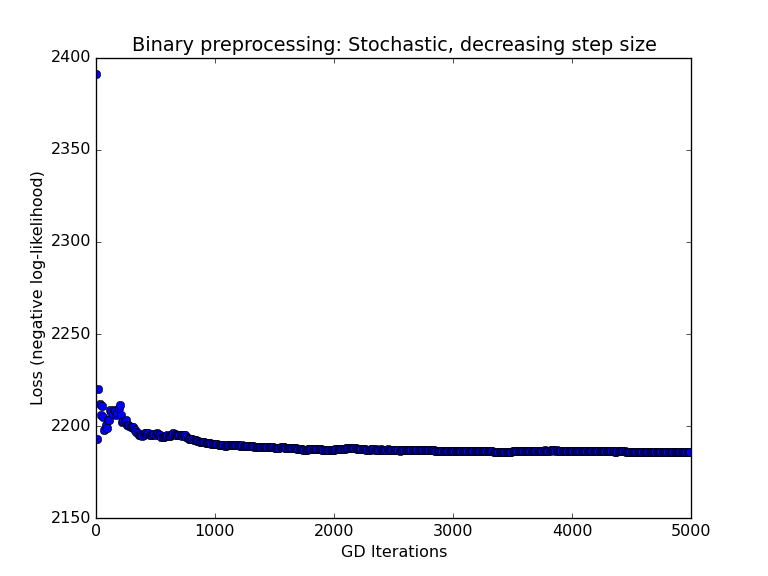
\includegraphics[scale=0.4]{images/p3_3_Binary} &
\end{tabular}
\end{enumerate}
%\begin{tabular}{cc}
%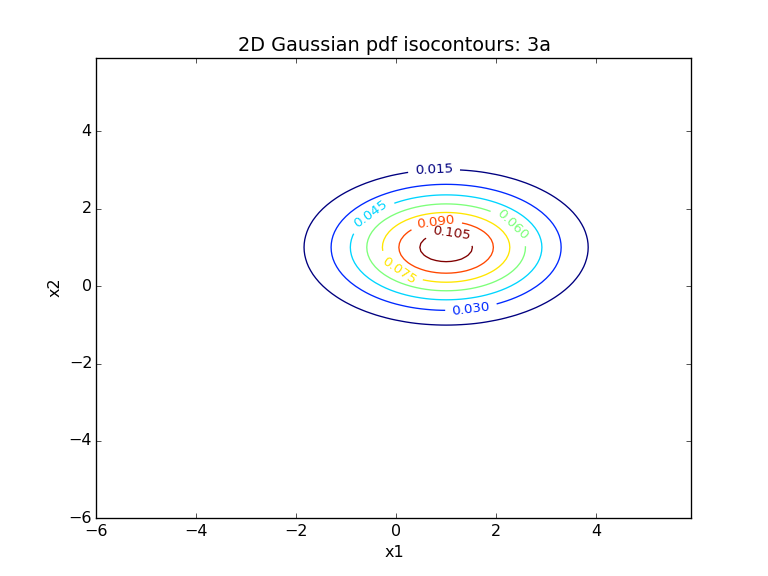
\includegraphics[scale=0.4]{images_hw3/p3a} & 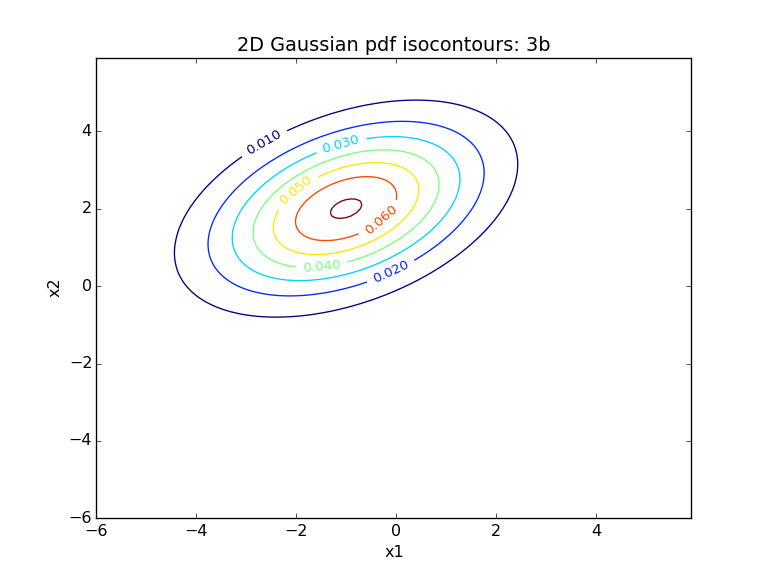
\includegraphics[scale=0.4]{images_hw3/p3b} \\
%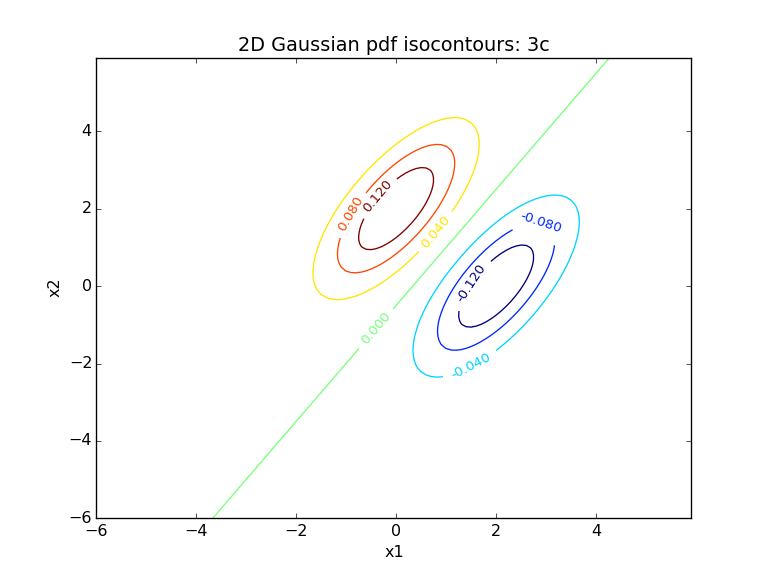
\includegraphics[scale=0.4]{images_hw3/p3c} & 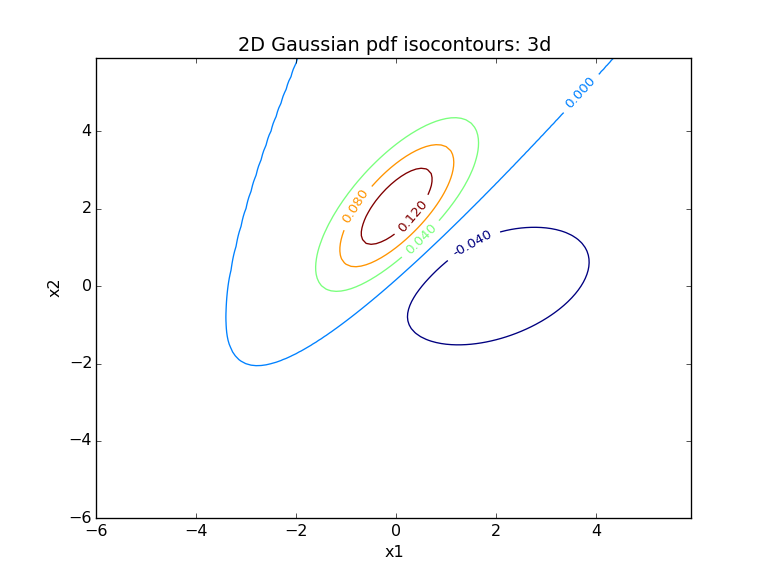
\includegraphics[scale=0.4]{images_hw3/p3d} \\
%\end{tabular}


\end{document}
